\documentclass[border=2pt]{standalone}

% Drawing
\usepackage{tikz}
\usepackage{pgfplots}
\pgfplotsset{compat=newest}
\usetikzlibrary{calc}

% Notation
\usepackage{physics}

% Styles
\tikzset{mass/.style={inner sep = 2pt}}

\begin{document}
	
	
	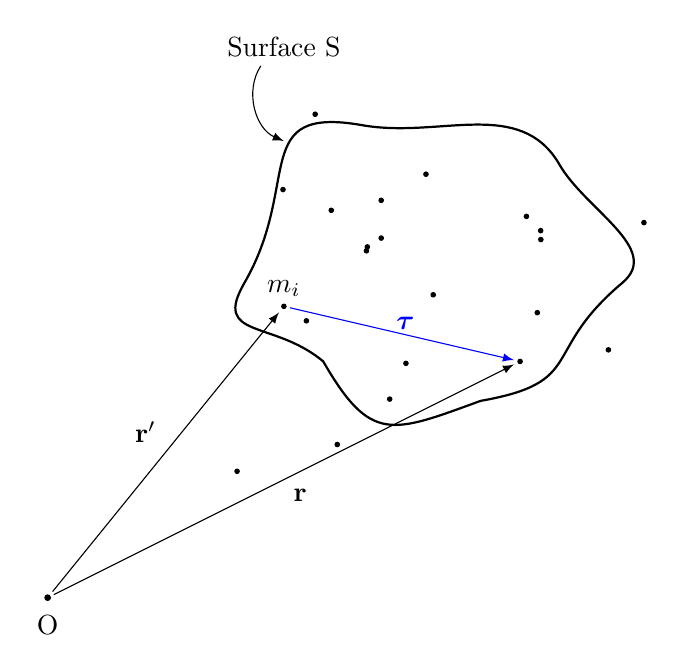
\begin{tikzpicture}
%		%Grid
%		\draw[thin, dotted] (0,0) grid (8,8);
%		\foreach \i in {1,...,8}
%		{
%			\node at (\i,-2ex) {\i};	
%		}
%		\foreach \i in {1,...,8}
%		{
%			\node at (-2ex,\i) {\i};	
%		}
%		\node at (-2ex,-2ex) {0};
		
		% Coordinates
		\node[mass] (O) at (0,0) {};
		\coordinate (A) at (3.5,3);
		\coordinate (B) at (5.5,2.5);
		\coordinate (C) at (7.3,4);
		\coordinate (D) at (6.5,5.5);
		\coordinate (E) at (4,6);
		\coordinate (F) at (2.5,4);
		\node[mass] (G) at (3,3.7) {};
		\node[mass] (H) at (6,3) {};
		%% Nodes
%		\foreach \i in {A,B,...,F}
%		{
%			\node at (\i) {\i};
%		}
		
		
		% Body
		\draw[thick] (A) to[out=-60, in=200, looseness=1.5] (B) to[out=10, in=220, looseness=1.5] (C) to[out=40, in=-60, looseness=1] (D) to[out=120, in=-10, looseness=1] (E) to[out=170, in=60, looseness=1.5] (F) to[out=240, in=140, looseness=1.5] cycle;
		
		% Masses
		% In the Body
		\foreach \i in {1,2,...,10}
		{
			\pgfmathsetmacro{\xcoor}{2*rand + 5} % x-coordinate
			\pgfmathsetmacro{\ycoor}{1.5*rand + 4} % y-coordiante 
				
			\draw[fill=black] (\xcoor, \ycoor) circle (0.8pt);
		}
		% Out of the Body
		\foreach \i in {1,2,...,10}
		{
			\pgfmathsetmacro{\xcoor}{2.7*rand + 5} % x-coordinate
			\pgfmathsetmacro{\ycoor}{2.4*rand + 4} % y-coordiante 
				
			\draw[fill=black] (\xcoor, \ycoor) circle (0.8pt);
		}
		\draw[fill=black] (G) circle (0.8pt);
		\draw[fill=black] (H) circle (0.8pt);
		
		% Nodes
		\node (s) at (3,7) {Surface $\mathrm{S}$};
		\node[above] at (G) {$m_i$};
		
		% Lines
		\draw[-latex] (O) -- (G) node [pos=0.5, above left] {$\vb{r}'$};
		\draw[-latex, blue] (G) -- (H) node [pos=0.6, above left] {$\vb*{\tau}$};
		\draw[-latex] (O) -- (H) node [pos=0.5, below right] {$\vb{r}$};
		\draw[-latex] (s) to[bend right=50] (3,5.8);
		
		% Point
		\draw[fill=black] (O) circle (1pt) node [below, shift={(0,-0.1)}] {$\mathrm{O}$};
	\end{tikzpicture}
	
\end{document}
